\documentclass[tikz,border=2pt]{standalone}
\usepackage{times}
\usetikzlibrary{positioning,arrows.meta,calc}
\begin{document}
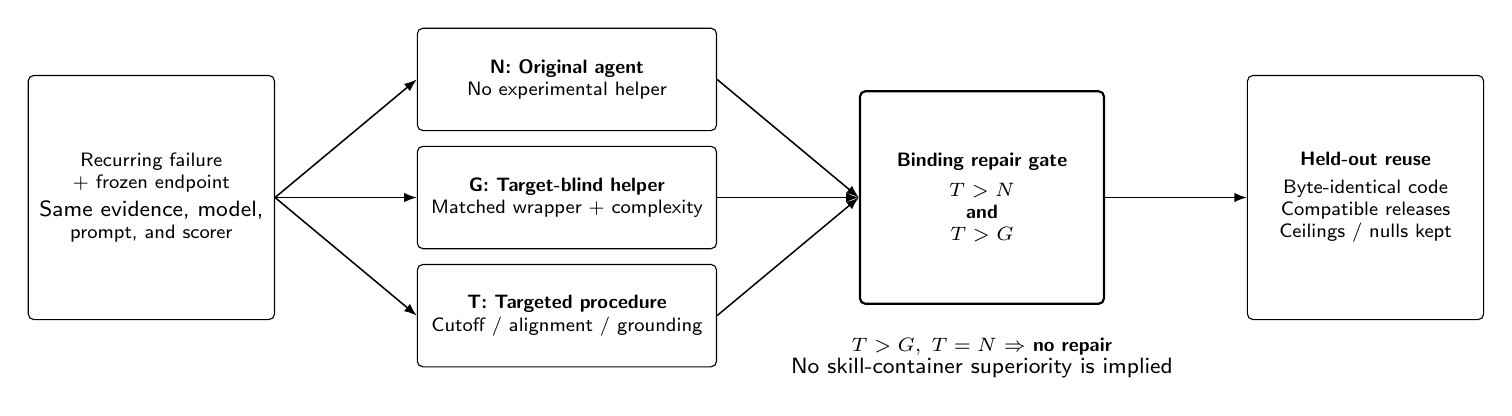
\begin{tikzpicture}[
  font=\sffamily\scriptsize,
  >={Latex[length=1.6mm]},
  box/.style={draw, rounded corners=2pt, align=center, inner sep=4pt, minimum height=13mm},
  arm/.style={box, minimum width=38mm},
  gate/.style={box, line width=0.8pt, minimum width=31mm, minimum height=27mm},
  flow/.style={->, line width=0.55pt}
]
\node[box, minimum width=31mm, minimum height=31mm] (src) {Recurring failure\\+ frozen endpoint\\[2pt]\footnotesize Same evidence, model,\\prompt, and scorer};

\node[arm, right=18mm of src, yshift=15mm] (n) {\textbf{N: Original agent}\\No experimental helper};
\node[arm, right=18mm of src] (g) {\textbf{G: Target-blind helper}\\Matched wrapper + complexity};
\node[arm, right=18mm of src, yshift=-15mm] (t) {\textbf{T: Targeted procedure}\\Cutoff / alignment / grounding};

\node[gate, right=18mm of g] (gate) {\textbf{Binding repair gate}\\[3pt] $T>N$\\\textbf{and}\\$T>G$};
\node[box, minimum width=30mm, minimum height=31mm, right=18mm of gate] (hold) {\textbf{Held-out reuse}\\[2pt] Byte-identical code\\Compatible releases\\Ceilings / nulls kept};

\draw[flow] (src.east) -- (n.west);
\draw[flow] (src.east) -- (g.west);
\draw[flow] (src.east) -- (t.west);
\draw[flow] (n.east) -- (gate.west);
\draw[flow] (g.east) -- (gate.west);
\draw[flow] (t.east) -- (gate.west);
\draw[flow] (gate.east) -- (hold.west);

\node[below=3mm of gate, align=center] {\textbf{$T>G,\;T=N$ $\Rightarrow$ no repair}\\\footnotesize No skill-container superiority is implied};
\end{tikzpicture}
\end{document}
